\documentclass[12pt]{article}
\usepackage{fancyhdr}
\pagestyle{fancy}
\usepackage{epsfig}
\usepackage{graphicx}
\graphicspath{{images/}}
\usepackage{listings}
\usepackage{color}

\definecolor{dkgreen}{rgb}{0,0.6,0}
\definecolor{gray}{rgb}{0.5,0.5,0.5}
\definecolor{mauve}{rgb}{0.58,0,0.82}

\lstset{frame=tb,
  language=Java,
  aboveskip=3mm,
  belowskip=3mm,
  showstringspaces=false,
  columns=flexible,
  basicstyle={\small\ttfamily},
  numbers=none,
  numberstyle=\tiny\color{gray},
  keywordstyle=\color{blue},
  commentstyle=\color{dkgreen},
  stringstyle=\color{mauve},
  breaklines=true,
  breakatwhitespace=true,
  tabsize=3
}


\begin{document}

\lhead{\textbf{Ian Benlolo}, ID 260744397-Comp 350\\Prof.Chang}
\rhead{Monday October $2^{nd}$ 2017}


\section {Question 1}
Here are some of my inputs/outputs. See appendix for code.\\
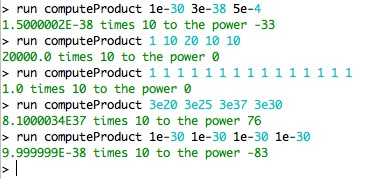
\includegraphics[width=3.4in]{q1}
\\
My test results all worked well. The last one outputs $9.99999e-113$ when it should be $1e-113$. This happens because of rounding in IEEE single format. 


\section{Question 2}
\subsection{A)}
My program (see appendix 2a for code, also attached with this doc in a .java file) gave the following results:\\
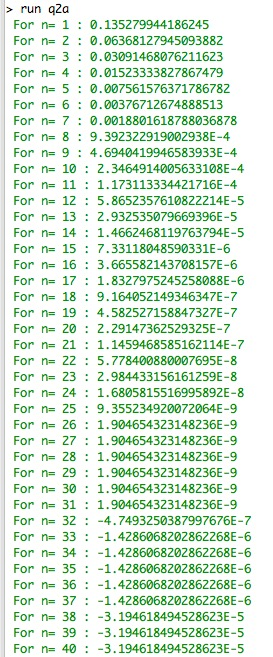
\includegraphics[width=2in]{q2a1}
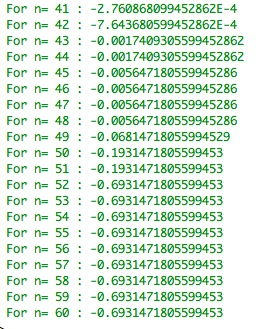
\includegraphics[width=2in]{q2a2}\\
The problem here is that it converges to $-ln(2)$ when it should be converging to $0$ since we our formula converges to $ln(2)$ so $ln(2)-ln(2)$ should be $0$ but it converges to $-ln(2)$. This happens due to discretization errors as well as cancellation errors. A computer can only do a finite number of evaluations while the function is continuous, and not discrete. 

\subsection{B)}
$$x_{n+1}=2^{n+1}(\sqrt{1+2^{-n}x_n}-1) \times \frac{\sqrt{1+2^{-n}x_n}+1}{\sqrt{1+2^{-n}x_n}+1}=\dots= \frac{2x_n}{\sqrt{1+2^{-n}x_n}+1}$$\\
Now, computing $x_n-ln(2)$ gives the following results:\\
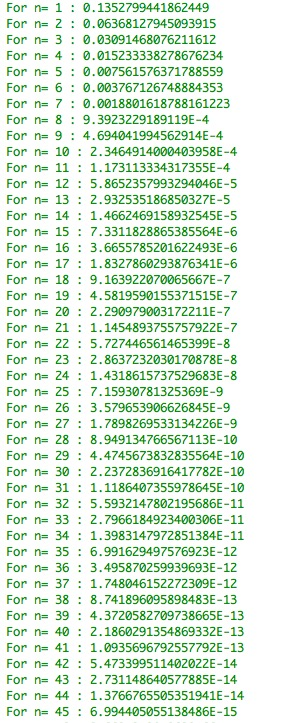
\includegraphics[width=2in]{q2ba}
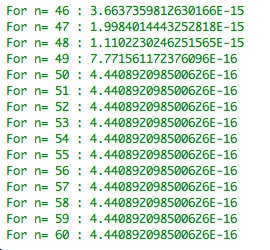
\includegraphics[width=2in]{q2bb}\\
Which effectively converges to 0 as we hoped. 


\newpage
\section{Appendix}
\subsection{1}
\begin{lstlisting}
import java.util.*;

public class computeProduct{
  public static void main(String[] args){
   int count=args.length;
   ArrayList<String> evenArg=new ArrayList<String>(Arrays.asList(args));
   
   if(count%2!=0){ //we will iterate through args in 2's so to make sure we 
     evenArg.add(0,"1"); //have an even number of args and if we dont
     count++;        // add a "1" at the end which wouldnt change anything 
   }
   int k=0;  //the value of K
   float finl=1; //the final result well will be printing
   
   
   for (int i=0; i<count-1; i+=2){ //iterate through every inputted number
     float x= Float.parseFloat(evenArg.get(i)); float y=Float.parseFloat(evenArg.get(i+1));  
     float temp;//start of by parsing args to floats 
     
     while (doesOverflow(x,y)){ //if the multiplication would overflow
       k++;
       if(x >= Float.MIN_NORMAL*10) x/=10; //to account for underflowing of x
       else y/=10; //wouldnt underflow because its x*y is overflowing..
     }
     while(doesUnderflow(x,y)){
       k--;
       if(x <= Float.MAX_VALUE/10) x*=10;
       else y*=10;
     }
     temp=x*y; //this does not overflow or underflow 
     if(doesOverflow(temp, finl) || doesUnderflow(temp, finl)){ //we will do the same as before
       while(doesOverflow(temp, finl)){//just now we add x and y to 'finl'
         k++;
         if(temp>=Float.MIN_NORMAL*10) temp/=10;
         else finl/=10;
         }
       while (doesUnderflow(temp, finl)){
         k--;
         if(temp<=Float.MAX_VALUE/10) temp*=10;
         else finl*=10;
         }
       }
     finl*=temp; //wont over/under flow at this point!
     }
   System.out.println(""+finl+" times 10 to the power "+k);
  }
  public static boolean doesOverflow(float x, float y){ //simply checks if multiplying
    if (x*y >= Float.MAX_VALUE) return true; //these two numbers will overflow
    else return false;
  }
  public static boolean doesUnderflow(float x, float y){ //same but for underflowing
    if (x*y<=Float.MIN_NORMAL)return true;
    else return false;
  }
}
\end{lstlisting}
\subsection{2}

\begin{lstlisting}
import java.math.*;

public class q2a{
  public static void main(String[] args){
    //Dynamic Programming method
    double[] x=new double[61];
    x[0]=1; //this is x_0
    for(int i=0; i<60; i++){
      x[i+1] = Math.pow(2,i+1)*(Math.sqrt(1+Math.pow(2,-i)*x[i])-1); 
    } //we just stored every value into an array using dynamic programming
    
    
    for(int i=1; i<61; i++){
      double y=x[i]-Math.log(2); // since x_0 is 1 its just ln(2)
      
      System.out.println(" For n= "+i+" : "+y);
      
    }
    
    double[] z=new double[61];       //q2b
    z[0]=1;
    for(int i=0; i<60; i++){
      z[i+1]=2*z[i]/(Math.sqrt(1+Math.pow(2,-i)*z[i])+1); 
      
    }
    System.out.println("q2b");
     for(int i=1; i<61; i++){
      double y=z[i]-Math.log(2);
      
      System.out.println(" For n= "+i+" : "+y);
      
    }
  }
}
\end{lstlisting}
\end{document}